%; whizzy chapter -dvi
% -initex iniptex -latex platex -format platex -bibtex jbibtex -fmt fmt
% $B0J>e(B whizzytex $B$r;HMQ$9$k>l9g$N@_Dj!#(B
 
%     Tokyo Debian Meeting resources
%     Copyright (C) 2012 Junichi Uekawa
%     Copyright (C) 2011 Nobuhiro Iwamatsu

%     This program is free software; you can redistribute it and/or modify
%     it under the terms of the GNU General Public License as published by
%     the Free Software Foundation; either version 2 of the License, or
%     (at your option) any later version.

%     This program is distributed in the hope that it will be useful,
%     but WITHOUT ANY WARRANTY; without even the implied warranty of
%     MERCHANTABILITY or FITNESS FOR A PARTICULAR PURPOSE.  See the
%     GNU General Public License for more details.

%     You should have received a copy of the GNU General Public License
%     along with this program; if not, write to the Free Software
%     Foundation, Inc., 51 Franklin St, Fifth Floor, Boston, MA  02110-1301 USA

%  preview (shell-command (concat "evince " (replace-regexp-in-string "tex$" "pdf"(buffer-file-name)) "&"))

%%$B$3$3$+$i%X%C%@3+;O!#(B

\documentclass[mingoth,a4paper]{jsarticle}
\usepackage{monthlyreport}

% $BF|IU$rDj5A$9$k!"Kh7nJQ$o$j$^$9!#(B
\newcommand{\debmtgyear}{2013}
\newcommand{\debmtgmonth}{11}
\newcommand{\debmtgdate}{16}
% started from zero:
% (let ((year 2013) (month 7)) (+ (* (- year 2005) 12) month -1))
\newcommand{\debmtgnumber}{106}

\begin{document}

\begin{titlepage}
\thispagestyle{empty}
% $B%?%$%H%k%Z!<%8(B:$BJT=8I,MW$JItJ,$O:G=i$N%^%/%m$KHt$P$9$3$H(B

\vspace*{-2cm}
$BBh(B\debmtgnumber{}$B2s(B $BEl5~%(%j%"(B Debian $BJY6/2q;qNA(B\\
\hspace*{-2cm}

\includegraphics{image2012-natsu/dotdeb.pdf}\\
\hfill{}\debmtgyear{}$BG/(B\debmtgmonth{}$B7n(B\debmtgdate{}$BF|(B

% $B$3$3$O%"%C%W%G!<%H$9$k$3$H(B
% $BA43QJ8;z$K$7$J$$$H%U%)%s%H$N%5%$%:$,9g$o$J$$$N$GCm0U(B
\rotatebox{10}{\fontsize{32}{32} {\gt $BFC=8#1!'(B $B#w#a#y#l#a#n#d$rF0$+$9(B}}

\rotatebox{10}{\fontsize{32}{32} {\gt $BFC=8#2!'(B $B%b%P%$%k4D6-9=C[(B}}

\vspace*{-2cm}
\hfill{}
\includegraphics[height=6cm]{image200502/openlogo-nd.eps}
\end{titlepage}

\newpage

\begin{minipage}[b]{0.2\hsize}
 \definecolor{titleback}{gray}{0.9}
 \colorbox{titleback}{\rotatebox{90}{\fontsize{80}{80} {\gt $B%G%S%"%sJY6/2q(B} }}
\end{minipage}
\begin{minipage}[b]{0.8\hsize}
\hrule
\vspace{2mm}
\hrule
\begin{multicols}{2}
\tableofcontents
\end{multicols}
\vspace{2mm}
\hrule
\end{minipage}

\dancersection{$B;vA02]Bj(B}{$B>e@n(B $B=c0l(B}

$B:#2s$N;vA02]Bj$O0J2<$G$9(B:
\begin{enumerate}
 \item wayland vs mir $B$K$D$$$F$*$b$&$3$H$r8l$C$F$/$@$5$$!#(B
\end{enumerate}
$B$3$N2]Bj$KBP$7$FDs=P$$$?$@$$$?FbMF$O0J2<$G$9!#(B
\begin{multicols}{2}
{\small
 
\begin{prework}{ $BLn<s(B }

$B8eH/$G$"$j$J$,$iM%0L@-$N$_$i$l$J$$(BMir$B$K0UL#$,$"$k$H$9$l$P!"$=$l$O(BCanonical$B$,%3%s%H%m!<%k2DG=$JE@$@$1$J$N$+$J$H$$$&5$$,$7$^$9!#(B

\end{prework}

\begin{prework}{ dictoss($B?yK\!!E5=<(B) }


\end{prework}

\begin{prework}{  $B@6LnM[0l(B }

$BIaCJ$"$^$j0U<1$7$?$3$H$,$J$+$C$?$N$G!"$3$l$r5$$KJY6/$G$-$l$P$H;W$$$^$9!#(B
\end{prework}

\begin{prework}{ mtoshi }

$B$5$C$Q$jJ,$+$j$^$;$s(B($BN^(B)
\end{prework}

\begin{prework}{ $B$^$($@$3$&$X$$(B }

$BL>A0$7$+<*$K$7$?$3$H$,$J$$$N$G!"$5$C$Q$jJ,$+$i$J$$!#(B
\end{prework}

\begin{prework}{ $BLnEg!!5.1Q(B }

wayland$B$b4hD%$C$?!*(Bmir$B$O<+J,$O$h$/$o$+$i$s$,!"4hD%$C$F$k!*(BX$B$bIi$1$F$J$$!*(B
$B$$$d!<!"$3$A$i$N@o$$$OL\$,$O$J$;$^$;$s%M!<!#2?;v$b6%AhAj<j$,$$$k$C$FNI$$$3$H$G$9%M!<!#(B
mir$B$H$NHf3S$O8!F$$7$?$3$H$J$$$N$G!"0c$$$K$D$$$FC/$+$h$m$7$/$*$M$,$$$7$^$9!#$$$:$l$K$7$F$b!"<+J,$H$7$F$O!"AH$_9~$_4^$a$F4JC1$KM7$Y$=$&$@$7!"Cf?H$9$C$4$$$o$+$j$d$9$$<BAu$G$"$k!"(Bwayland$B$H$7$P$i$/5:$l$h$&$H;W$C$F$^$9!#(B

$B"((Bmir$B$OD4$Y$F$J$$$h(B?

\end{prework}

\begin{prework}{ $B>e@n=c0l(B }

x11$B$N%W%m%H%3%k$O2~NI$NM>CO$,$"$k$H;W$&$N$G4hD%$C$F3+H/$,?J$_6%Ah$,$"$k$N$O9%$^$7$$$H;W$$$^$9!#(B
\end{prework}

}
\end{multicols}

\dancersection{Debian Trivia Quiz}{$B>e@n=c0l(B}

$B$H$3$m$G!"$_$J$5$s(B Debian $B4XO"$NOCBj$K$*$$$D$$$F$$$^$9$+!)(BDebian$B4XO"$NOC(B
$BBj$O%a!<%j%s%0%j%9%H$r$h$s$G$$$k$HDI@W$G$-$^$9!#$?$@$h$s$G$$$k$@$1$G$O$O(B
$B$j$"$$$,$J$$$N$G!"M}2rEY$N%F%9%H$r$7$^$9!#FC$K0l?M$@$1$G$O0UL#$,$o$+$i$J(B
$B$$$H$3$m$b$"$k$+$bCN$l$^$;$s!#$_$s$J$G0l=o$KFI$s$G$_$^$7$g$&!#(B

$B:#2s$N=PBjHO0O$O(B\url{debian-devel-announce@lists.debian.org} $B$d(B \url{debian-devel@lists.debian.org}$B$KEj9F$5$l$?(B
$BFbMF$H(BDebian Project News$B$+$i$G$9!#(B

\begin{multicols}{2}
% %; whizzy-master ../debianmeetingresume201311.tex
% $B0J>e$N@_Dj$r$7$F$$$k$?$a!"$3$N%U%!%$%k$G(B M-x whizzytex $B$9$k$H!"(Bwhizzytex$B$,MxMQ$G$-$^$9!#(B
%

\santaku
{alioth $B$K$J$K$,$*$-$?$+(B}
{$B7|>^$,$"$?$C$?(B}
{RAID$B$N%O!<%I%G%#%9%/$,(B2$B8D2u$l$?(B}
{$B?7%"!<%-%F%/%A%c$K0\9T$7$?(B}
{B}
{RAID$B$N%O!<%I%G%#%9%/$,(B2$B$D2u$l$F%U%!%$%k%7%9%F%`$,2u$l$?$=$&$G$9!#(B}

\santaku
{DSA$B$,(BDPL$B$N>5G'$J$/;H$($kM=;;$O$$$/$i$+(B}
{\$ 0}
{\$ 100}
{\$ 400}
{C}
{$B%G%#%9%/$,2u$l$F8r49$9$k$N$K$b(BDPL$B$r$^$?$J$$$H$$$1$J$+$C$?$N$+$J!#(B}

\santaku
{Jessie $B$N%U%j!<%:$O$$$D$+(B}
{2013$BG/(B11$B7n(B5$BF|(B}
{2014$BG/(B11$B7n(B5$BF|(B}
{2015$BG/(B11$B7n(B5$BF|(B}
{A}
{$B$"$l!"$b$&%U%j!<%:$7$F$k!)(B}

\santaku
{policy 3.9.5.0$B$K$h$k$H%P%$%J%j%Q%C%1!<%8Fb$N%U%!%$%kL>$N%(%s%3!<%G%#%s%0$O$J$K$+(B}
{UTF-8}
{Latin-1}
{sjis}
{A}
{$B$H$&$H$&(BASCII$B0J30$,G'$a$i$l$k$h$&$K$J$j$^$7$?$+!#(B}

\end{multicols}

\dancersection{$B:G6a$N(BDebian$B4XO"$N%_!<%F%#%s%0Js9p(B}{$B>e@n=c0l(B}
\subsection{$BEl5~%(%j%"(BDebian$BJY6/2q(B103$B2sL\Js9p(B}

\subsection{OSC $BEl5~(B/Fall}


% (query-replace-regexp "<.*?>" "")
% (query-replace-regexp "^[	 ]\+" "")

%-------------------------------------------------------------------------------
\dancersection{wayland$B$rF0$+$9(B}{$BLnEg(B $B5.1Q(B}
%-------------------------------------------------------------------------------
\index{wayland}

\subsection{wayland}
 wayland$B$H$O!"(BKristian Hoegsberg$B$5$s(B(oe$B$O%9%H%m!<%/IU$-(Bo)$B$,Cf?4$H$J$C$F:n$C$F$$$k%G%#%9%W%l%$%5!<%P!<$N%W%m%H%3%k$N$3$H$G$9!#(Bwayland$B%W%m%H%3%k$r07$($k%G%#%9%W%l%$%5!<%P!<$H$7$F(Bweston$B$,$"$j$^$9!#(B 

 $B=>Mh$+$i$"$k(BUnix$B$GM-L>$J%G%#%9%W%l%$%5!<%P!<$N%W%m%H%3%k$H$7$F$O!"(BX$B%W%m%H%3%k$,$"$j!"(BX$B%W%m%H%3%k$r07$($k%G%#%9%W%l%$%5!<%P!<$K(BX$B$,$"$j$^$9!#$7$+$7$J$,$i!"(BX$B$O(B1984$BG/:"$N@_7W$+$i;O$^$C$F!"$:$C$H%O!<%I$N?J2=$K$"$o$;$F$D$.$O$.$7$F$-$?$?$a!"$$$m$$$m<BAu$H5!G=$KL5M}$,@8$8$F$$$^$9!#(Bwayland$B$O!"(BX$B$KHf$Y$F!"05E]E*$K@vN}$5$l$?@_7W$G!"%7%s%W%k$K!"%W%m%H%3%k$H%G%#%9%W%l%$%5!<%P!<$r<B8=$7$?$b$N$H$J$j$^$9(B\cite{real-wayland-X}$B!#(B


\subsection{weston$B$NF0$$$F$$$kMM;R(B}

$B!!(Bweston$B$NF0$$$F$$$kMM;R$r:\$;$^$9!#(B

\begin{minipage}{0.5\hsize}
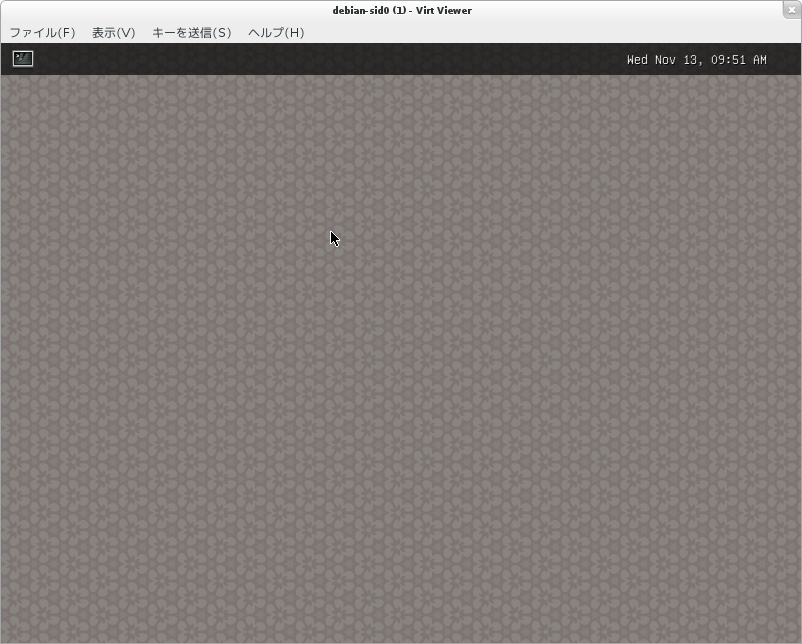
\includegraphics[width=0.8\hsize]{image201311/weston-1st-launch.png}
\end{minipage}
\begin{minipage}{0.5\hsize}
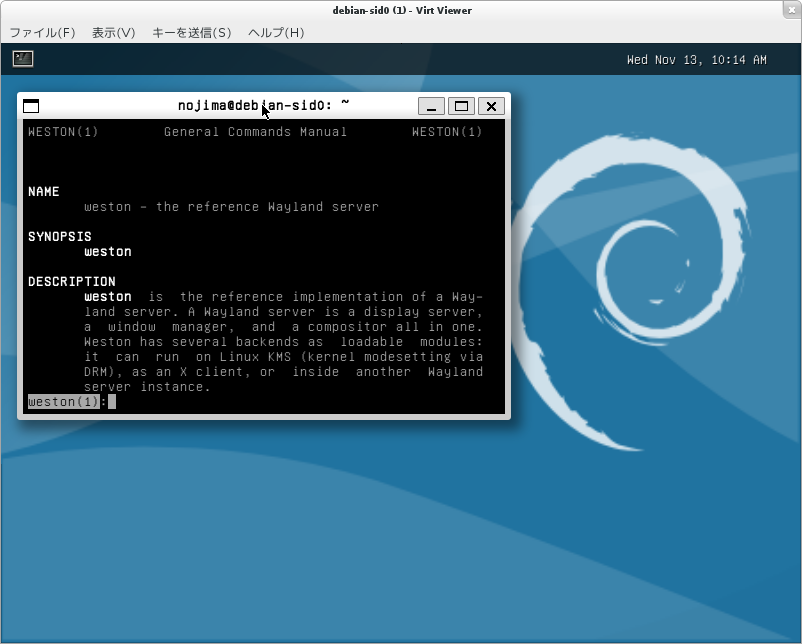
\includegraphics[width=0.8\hsize]{image201311/weston-2nd-launch.png}
\end{minipage}

\subsection{weston$B$NBP1~=PNO%G%P%$%9(B}

 weston$B$NBP1~$G$-$k=PNO%G%P%$%9$OI=(B\ref{tab:debian-weston-backends}$B$H$J$j$^$9!#(B

\begin{table}[ht]
\begin{center}
\begin{tabular}{|l|p{4cm}|p{4cm}|p{3cm}|l|}
\hline 
$B9`HV(B&$B=PNO%G%P%$%9(B&$B%P%C%/%(%s%IL>(B&$B%Q%C%1!<%8$KEk:\:Q(B&$BHw9M(B\\
\hline \hline
1& DRM/KMS & drm-backend.so & $B!{(B & \\
2& FrameBuffer & fbdev-backend.so & $B!{(B & \\
3& X & x11-backend.so & $B!{(B & \\
4& Wayland & wayland-backend.so & $B!{(B & \\
5& Headless & headless-backend.so & $B!{(B & \\
5& Rassberry Pi & rpi-backend.so & $B!_(B & \\
6& RDP & rdp-backend.so & $B!_(B & \\
\hline
\end{tabular}
\caption{\label{tab:debian-weston-backends}$B=PNO%G%P%$%9$H(Bweston$B$NBP1~>u67(B}
\end{center}
\end{table}

\subsection{debian$B$G$N(Bweston$B2TF/$N$?$a$N2<=`Hw(B}
\label{sec:pre-requisite}
debian$B$G(Bweston$B$rF0:n$5$;$k$K$O!"0J2<$N2<=`Hw$,I,MW$G$9!#(B

\begin{description}
\item [Step 1.] weston$B$NF3F~$r$7$^$9!#(B
\begin{commandline}
# aptitude install weston
\end{commandline}
\item [Step 2.] systemd$B%Q%C%1!<%8$rF3F~$9$k$J$I$7$F!"4D6-JQ?t(BXDG\_RUNTIME\_DIR$B$,@_Dj$5$l$k$h$&$K$7$^$9!#(B
\begin{commandline}
# aptitude install systemd
\end{commandline}
\item [Step 3.] weston-launch$B$K%f!<%6$r2C$(!"%m%0%$%s$7$J$*$7$^$9!#(B
\begin{commandline}
# usermod -a -G weston-launch <your-login-id>
...$B=EMW!'$3$N8e%m%0%$%s$7$J$*$9(B...
\end{commandline}
\item [Step 4.] $B4D6-JQ?t(BXDG\_RUNTIME\_DIR$B$,@_Dj$5$l$F$$$k$+3N$+$a$^$9!#$J$*!"2?$i$+$NM}M3$G!"(Bsystemd$B%Q%C%1!<%8IUB0$N(Bsystemd-logind$B$,F0:n$7$J$$Ey$NM}M3$K$h$j!"(BXDG\_RUNTIME\_DIR$B$,@_Dj$5$l$F$$$J$$$N$G$"$l$P!"(Bexport XDG\_RUNTIME\_DIR=/tmp$B$J$I$7$F=q$-9~$_$,2DG=$J%G%#%l%/%H%j$r;XDj$7$F$*$-$^$9!#(B
\begin{commandline}
[1] systemd-logind$B$,L5;vF0$$$F$$$k>l9g"-(B
$ env| fgrep XDG_RUNTIME_DIR
XDG_RUNTIME_DIR=/run/user/1000

[2] systemd-logind$B$,2?$i$+$NM}M3$GF0:n$7$F$$$J$$>l9g"-(B
$ env| fgrep XDG_RUNTIME_DIR
...$B$J$K$bI=<($5$l$J$$(B...
$ export XDG_RUNTIME_DIR=/tmp
\end{commandline}
%$
\end{description}

\subsection{$B$=$N#1(B:X$B>e$GF0$+$7$F$_$k(B}

 $B0lHV4JC1$KF0$+$;$^$9!#(BX$B$N%?!<%_%J%k%=%U%H>e$G!"(B

\begin{commandline}
weston
\end{commandline}

$B$H$9$k$@$1$G!"(Bx11-backend.so$B$,FI$_9~$^$l!"(B
weston$B$NAk$,3+$-!"(Bweston$B$,F0:n$r3+;O$7$^$9!#(B

$BDd;_$9$k;~$O!"(Bweston$B$r5/F0$7$F$$$k%?!<%_%J%k$G!"(BCtrl-C$B$r2!2<$7$^$9!#(B

\subsubsection{X$B>e$GF0$+$7$F$_$k;~$NCm0UE@(B}

 $B2?8N$+!"<j85$N(Bnvidia$B@=%0%i%U%#%/%9%+!<%I$K$F!"(Bnon-free$B$N(Bnvidia$B%I%i%$%P$r(B
$B;H$C$F$$$k$H!"2hLL??$C9u$N%&%#%s%I%&$,3+$$$F$7$^$$$^$7$?!#(B--use-pixmap$B$r;XDj(B
$B$7$F(Bweston$B$r5/F0$7$F!"(Bweston$B$,(BEGL$BEy$N%O!<%I%&%'%"%"%/%;%i%l!<%7%g%s$r(B
$BMxMQ$7$J$$$h$&$K$7$F$bF1MM$@$C$?$j$7$^$9!#0lJ}$G!"(Bintel$B@=$N%0%i%U%#%/%9(B
$B%A%C%W$r:\$;$F$$$k%N!<%H(BPC$B>e$G$OLdBj$J$/F0:n$7$^$7$?!#(B

$B!!$3$A$i$N860x$O$^$@$D$+$a$F$$$^$;$s!#(B

\subsection{$B$=$N(B2:KMS/DRM$B$GF0$+$7$F$_$k(B}

$B!!(Bintel$B$N%0%i%U%#%C%/%9%A%C%W$,Ek:\$5$l$F$$$k(BPC($BNc!'%N!<%H(BPC$B$H$+!K(B
$B$G$"$l$P!"(Blinux$B$N(BKMS/DRM$B%I%i%$%P$GF0:n$7$^$9!#$^$?!"(B
AMD/Nvidia$B$N%0%i%U%#%/%9%A%C%W$G$"$l$P!"(Blinux$B$N(BKMS/DRM$B%I%i%$%P$N(B
radeon/nouveau$B%I%i%$%P$GF0:n$9$k$H;W$o$l$^$9$,!"<+J,$OL$I>2A$G$9!#(B
$B$I$J$?$+(Bradeon/nouveau$B$GF0:n$7$?J}$,$$$i$C$7$c$l$P65$($F$/$@$5$$!#(B

\begin{description}
\item [Step 1.] $B%0%i%U%#%+%k$J%m%0%$%s2hLL$,=P$F$$$k$h$&$G$"$l$P!"$3$A$i$rDd;_$5$;$^$9!#(B\\
$BNc!'(Bgdm3$B$,N)$A>e$,$C$F$$$k>l9g$N;_$aJ}(B
\begin{commandline}
Ctrl-Alt-F1$BEy$r2!2<$7$F%3%s%=!<%k$K@Z$jBX$($k(B
$ su
# service gdm3 stop
\end{commandline}
%$
\item [Step 2.] KMS/DRM$B%I%i%$%P$,M-8z$G$"$k$3$H$r3N$+$a$^$9!#(B
\begin{commandline}
$ lsmod | egrep '(i915|radeon|nouveau)'
...(i915/radeon/nouveau$B$N$I$l$+$NJ8;zNs$,=P$l$P(BOK)...
\end{commandline}
%$
\item [Step 3] weston$B$rF0$+$7$^$9!#(B
\begin{commandline}
$ weston-launch
\end{commandline}
%$
\end{description}

\subsubsection{KMS/DRM$B>e$GF0$+$7$F$_$k;~$NCm0UE@(B}

 linux$B$N(BKMS/DRM$B%I%i%$%P$O!"(Bi915/radeon/nouveau$B0J30$OF0:n$9$k$+$I$&$+$O@5D>$d$C$F$_$J$$$HJ,$+$j$^$;$s!#(B

$B!!Nc$($P!"(Bdebian$B$K$F!"2>A[2=5;=Q$N(BKVM$B$G$O(Bcirrus$B%A%C%W%;%C%HMQ$N(BKMS/DRM$B%I%i%$%P$,(Bvirt-viewer$B$N85$G;H$($k$N$G$9$,!"(Bweston$B$O(Begl$BB&(Bcirrus$BL$BP1~$K$h$k%(%i!<$b$7$/$O!"(BSegfault$B$GMn$A$F$7$^$&$?$a$I$&$K$bF0:n$7$^$;$s$G$7$?!#$3$A$i$b860x$,<+J,$G$O@53N$K$D$+$a$F$$$^$;$s!#(B

\subsection{$B$=$N(B3.FrameBuffer$B%G%P%$%9>e$GF0$+$7$F$_$k(B}

 linux$B$N(BFrameBuffer$B%G%P%$%9>e$GF0$+$7$F$_$^$9!#:#$N$H$3$m2>A[2=5;=Q$N(BKVM$B>e$GF0$+$9$N$KJXMx$G$9!#$3$3$G$O!"<B:]$K(BKVM$B$r;H$C$FF0$+$7$^$9!#(B

 $B$J$*!"BgJQ;DG0$J$3$H$K!"8=:_$N(Bdebian sid$B$GF3F~$G$-$k(Bweston$B%Q%C%1!<%8$N%P!<%8%g%s(B1.3.0$B$G$O!"2>A[C<Kv@)8f$K4X$9$k(Bupstream$BB&$N%P%0$N$?$a$K!"(BFrameBuffer$B%G%P%$%9$G$OF0:n$7$^$;$s!#9,$$!"$3$A$i$N%P%0$,=$@5$5$l$?!"(Bweston-1.3.1$B$,%j%j!<%9$5$l$^$7$?$N$G!"$3$3$G$O!"$3$N%P!<%8%g%s$r4J0WE*$K(Bdebian$B%Q%C%1!<%82=$7$FF3F~$7$^$9!#(B

\begin{description}
\item [Step 1.]  weston$B$rF0$+$9BP>]$N(Bdebian sid$B$r(BKVM$B$r;H$C$F%$%s%9%H!<%k$7$^$9!#$J$*!"(BKVM$B%[%9%H(BOS$BB&$N(Bdebian$B5!$N(Bbr0$B$O%$%s%?!<%M%C%H$K@\B3$G$-$k$h$&$K@_Dj$5$l$F$$$k$b$N$H$7$^$9!#(Bbr0$B$N%;%C%H%"%C%W$K$D$$$F!">\$7$/$O(B\cite{kde-devel-debian}$B$r;2>H$7$F$/$@$5$$!#(B
\begin{commandline}
# aptitude install libvirt-bin virtinst
# qemu-img create -f raw /var/lib/libvirt/images/debian-sid0 10G
# wget http://cdimage.debian.or.jp/7.2.0/multi-arch/iso-cd/debian-7.2.0-amd64-i386-netinst.iso
# virt-install --connect=qemu:///system -n debian-sid0 --ram 512  --cdrom /home/yours/debian-7.2.0-amd64-i386-netinst.iso \
  --disk /var/lib/libvirt/images/debian-sid0,bus=virtio,size=10,format=raw,cache=writeback \
  --bridge=br0,model=virtio --vnc --hvm --accelerate
\end{commandline}

 $B$J$*!"%$%s%9%H!<%k$N:]$N@_Dj$OI=(B\ref{tab:inst-settings}$B$N$H$*$j$r2>Dj$7$^$9!#(B

\begin{table}[ht]
\begin{center}
\begin{tabular}{|l|p{5cm}|p{7cm}|l|}
\hline 
$B9`HV(B&$B@_Dj9`L\(B&$B;XDjFbMF(B&$BHw9M(B\\
\hline \hline
1&select a language& Japanese& \\
2&$B>l=j$NA*Br(B&$BF|K\(B&\\
3&$B%M%C%H%o!<%/$N@_Dj(B&$B<jF0@_Dj!#(B IP:192.168.0.2, Netmask:255.255.255.0, Gateway:192.168.0.1, Host$BL>(B:debian-sid0& \\
4&$B%Q%C%1!<%8%^%M!<%8%c$N@_Dj(B&$B%_%i!<(B:$BF|K\(B,$B%_%i!<%5%$%H(B:ftp.jp.debian.org, HTTP$B%W%m%-%7!'6uMs(B&\\
5&$B%=%U%H%&%'%"$NA*Br(B&SSH$B%5!<%P!<!"I8=`%7%9%F%`%f!<%F%#%j%F%#$N$_A*Br!#$"$H$O$9$Y$F2r=|!#(B& \\
\hline
\end{tabular}
\caption{\label{tab:inst-settings}$B%$%s%9%H!<%i$GA*Br$9$k9`L\(B}
\end{center}
\end{table}

\item [Step 2.] $B%$%s%9%H!<%k40N;$7$?$i!"$9$0$K(Bdebian sid$B$X%"%C%W%0%l!<%I$7$^$9!#(B

\begin{commandline}
debian-sid0$B$K%m%0%$%s$N8e!"(B
debian-sid0 $ su
debian-sid0 # cat > /etc/apt/sources.list
deb http://ftp.jp.debian.org/debian/ sid main contrib non-free
deb-src http://ftp.jp.debian.org/debian/ sid main contrib non-free
<ctrl+d>$B$r2!2<(B
debian-sid0 # aptitude update;aptitude full-upgrade;aptitude clean
\end{commandline}
%$

\item [Step 3.] weston-1.3.1-1$B%Q%C%1!<%8$r:n$C$FF3F~$7$^$9!#(B

\begin{commandline}
debian-sid0 # aptitude build-dep weston/sid
debian-sid0 # aptitude install libxcb-composite0-dev fakeroot
debian-sid0 # exit
debian-sid0 $ mkdir weston weston-work
debian-sid0 $ cd weston
debian-sid0 $ apt-get source weston/sid
debian-sid0 $ cd ../weston-work
debian-sid0 $ wget -O weston_1.3.1.orig.tar.gz \
  http://cgit.freedesktop.org/wayland/weston/snapshot/weston-1.3.1.tar.gz
debian-sid0 $ tar xzf weston_1.3.1.orig.tar.gz
debian-sid0 $ cd weston-1.3.1
debian-sid0 $ tar xzf ../../weston/weston_1.3.0-1.debian.tar.gz
debian-sid0 $ cd debian; 
debian-sid0 $ patch -p1 <<__HERE
--- debian.org/changelog        2013-10-11 20:04:50.000000000 +0900
+++ debian/changelog    2013-11-12 14:48:36.219299000 +0900
@@ -1,3 +1,9 @@
+weston (1.3.1-1) unstable; urgency=low
+
+  * update to upstream
+
+ -- your name <foo@bar.com>  Fri, 11 Nov 2013 12:34:56 +0900
+
 weston (1.3.0-1) unstable; urgency=low
 
   [ Sven Joachim ]
diff -ru debian.org/control debian/control
--- debian.org/control  2013-10-11 19:58:17.000000000 +0900
+++ debian/control      2013-11-12 14:49:32.347299000 +0900
@@ -35,6 +35,7 @@
  libpam0g-dev,
  libvpx-dev,
  libsystemd-login-dev,
+ libxcb-composite0-dev,
 Standards-Version: 3.9.4
 Homepage: http://wayland.freedesktop.org/
 Vcs-Git: git://anonscm.debian.org/pkg-xorg/wayland/weston
__HERE
debian-sid0 $ cd ..
debian-sid0 $ env DEB_BUILD_OPTIONS='noopt nostrip' \
   dpkg-buildpackage -rfakeroot -us -uc 2>&1 | tee ../build.log
debian-sid0 $ cd ..
debian-sid0 $ su
debian-sid0 # dpkg -i ./weston_1.3.1-1_amd64.deb
\end{commandline}

\item [Step 3.]  \ref{sec:pre-requisite}$B>O$N(BStep 2.$B!A(BStep 4.$B$K5-:\$N2<=`Hw$r$7$F$*$-$^$9!#(B(Step 1.$B$O@h$[$I9=C[$7$?(Bweston$B%Q%C%1!<%8$,F3F~:Q$_$G$9$N$GITMW$G$9!K(B


\item [Step 4.] FrameBuffer$B$N%;%C%H%"%C%W$r$7$^$9!#$J$*(Bweston$B$rF0$+$9$?$a$K$O!"(Bcolor depth$B$O(B24bit$B$G$J$1$l$P$J$j$^$;$s!#(B
\begin{commandline}
debian-sid0 # aptitude install fbset
debian-sid0 # modprobe cirrusfb
debian-sid0 # fbset -g 800 600 800 600 24
\end{commandline}

\item [Step 5.] $B0lHL%f!<%6$K$J$j!"(Bweston$B$r5/F0$7$^$9!#(B
\begin{commandline}
debian-sid0 # exit 
debian-sid0 $ weston-launch -- --backend=fbdev-backend.so --log=weston.log
\end{commandline}
%$
\end{description}

\subsection{weston$B$N%+%9%?%^%$%:(B}

 weston$B$O%G%U%)%k%H$N$^$^$@$H>/$7<d$7$$2hLL$J$N$G!"$A$g$C$H%+%9%?%^%$%:$7$F$_$^$9!#%+%9%?%^%$%:$O!p(BHOME/.config/weston.ini$B$K$$$m$$$m5-:\$9$k$H!"$$$m$$$m$H%+%9%?%^%$%:$G$-$^$9!#$3$3$G$OJI;f$rF~$l!"%&%#%s%I%&%]%C%W%"%C%W$,%"%K%a!<%7%g%s$9$k$h$&$J%+%9%?%^%$%:$r$7$F$_$^$9!#(B
\begin{commandline}
$ cat >.config/weston.ini$B!!(B<<__HERE 
[shell]
background-image=/usr/share/images/desktop-base/spacefun-grub.png
background-type=tile
locking=true
animation=zoom
binding-modifier=ctrl

[launcher]
icon=/usr/share/weston/terminal.png
path=/usr/bin/weston-terminal
__HERE
\end{commandline}
%$

\subsection{weston$B$N9=B$(B}

 $B?^(B\ref{fig:wayland-internal}$B$K(Bwayland$B%"%W%j%1!<%7%g%s$H(Bweston$B$N9=B$$r:\$;$^$9!#(B

\begin{figure}[H]
\begin{center}
 \includegraphics[width=0.8\hsize] {image201311/wayland-internal-schema.eps}
 \caption{wayland$B%"%W%j%1!<%7%g%s$H(Bweston}
\label{fig:wayland-internal}
\end{center}
\end{figure}

 $BFCD'$H$7$F!"(B
\begin{itemize}
\item $B4pK\E*$K%"%W%j%1!<%7%g%sB&$b4^$a$F!"%m!<%+%k%7%9%F%`$GIA2h$r9T$&$3$H$rA0Ds$K$7$?:n$j$K$J$C$F$$$^$9!#(B
\item cairo/mesa/xkbcommon$BEy$r:GBg8BMxMQ$7$F!"(Bweston$B<+BN$OHs>o$K%7%s%W%k$J@_7W$K$J$C$F$$$^$9!#(B
\item $B%W%m%;%9$N%f!<%68"8B$r@)8B$9$k$?$a!"(Bweston-lanch$B$K$O(Broot$B8"8B$,:GDc8BI,MW$JItJ,$N$_$NA`:n$r!"(Bweston$B$O0lHL%f!<%6$G$N8"8B$K$h$kF0:n$r$9$k$h$&$K!"8"8B$,J,3d$5$l$F$$$^$9!#$J$*!"8=:_$N<BAu$G$O(Bweston-launch$B$OA`:n!&%*!<%W%s:Q$_$NC<Kv$N(BFileDiscriptor$B$H!"%G%P%$%9%U%!%$%k$N(BFile Descriptor$B!"(Bweston-launch$B$X$N%7%0%J%k$r!"(Bweston$B$N5a$a$K1~$8$F0z$-EO$95!G=$,<BAu$5$l$F$$$^$9!#(B
\end{itemize}
\subsection{$B$=$NB>(B}

 debian$B$GMxMQ$G$-$k(Bweston/wayland$B$K$O$A$g$C$H$7$?%/%;$,$"$j$^$9!#(B

 \begin{itemize}
\item Xwayland$B$,F0:n$7$^$;$s!#$3$l$O(Bweston$B$,5/F0$9$k(BX$B$K(Bwayland$BMQ$N(BI/F$B$rEk:\$9$k%Q%C%A$,E&MW$5$l$F$$$J$1$l$P$J$i$J$$!J(BX$B5/F0;~$K(B-wayland$B%*%W%7%g%s$,;H$($J$1$l$P$J$i$J$$!K$N$G$9$,!"$3$A$i$OL$$@(BX$B$N%Q%C%1!<%8$K4^$a$i$l$F$$$J$$0Y$H$J$j$^$9!#$J$*!"(B2013/10$B:"$K$3$A$i$N(Bdebian$B%Q%C%1!<%8MQ$N%Q%C%A$,(Bdebian-x$B$N(BML$B$KN.$l$F$$$^$7$?!#(B
\item gtk$BEy$NM-L>$J%D!<%k%-%C%H$O(Bwayland$BL$BP1~$N>uBV$G$9!#(B
 \end{itemize}

\subsection{$B$*$o$j$K(B}

$B!!<!4|%G%#%9%W%l!<%5!<%P!<$K$J$k$+$b$7$l$J$$(Bweston$B$H(Bwayland$B$K$D$$$F!"$$$m$$$m;n$7$F$_$^$7$?!#%W%m%0%i%`K\BN$OHs>o$K>.$5$$%W%m%0%i%`$G$9$7!"H/E8ES>e$G$9$N$G!"$$$8$C$F$_$h$&$H$$$&J}$O!":#$J$i$?$d$9$/2~B$(B/$B2r@O$7J|Bj$N=\$J;~$G$9!#(BHack$B$NBP>]$K$<$R!#(B

\begin{thebibliography}{0}
  \bibitem{real-wayland-X}
    {\footnotesize{
       Daniel Stone,``The real story behind Wayland and X'',linux.conf.au 2013,
       \url{http://people.freedesktop.org/~daniels/lca2013-wayland-x11.pdf},
       \url{http://www.youtube.com/watch?v=RIctzAQOe44}
       }}
  \bibitem{kde-devel-debian}
    {\footnotesize{
       $BLnEg(B $B5.1Q(B,$B!V(BDebian$B3+H/<T$N(BKDE$B4D6-$"$l$3$l!W(B,$BBh(B85$B2sEl5~%(%j%"(BDebian$BJY6/2q;qNA(B,
       \url{http://tokyodebian.alioth.debian.org/pdf/debianmeetingresume201202.pdf}
       }}
\end{thebibliography}

%-------------------------------------------------------------------------------
\dancersection{tramp$BF~Lg(B}{$B>e@n=c0l(B}
%-------------------------------------------------------------------------------
\index{tramp}

\subsection{emacs$B$G%j%b!<%H%U%!%$%kJT=8$9$k(BTramp$B$N$9$9$a(B}

$B%j%b!<%H%5!<%P$G%U%!%$%k$NJT=8$O$I$&$7$F$$$^$9$+!)(Bmosh$B$r;H$C$F$$$k!)(B
sshfs$B$r;H$C$F$$$k!)$$$m$$$m$"$k$H;W$$$^$9$,(Bmosh$B$r;H$&$H%m!<%+%k$N%U%!%$%k(B
$B$H07$$$,JQ$o$C$F$7$^$$!"%j%b!<%H$N(Bvi$B$@$C$?$j(Bemacs$B$r;H$C$FJT=8$9$k$3$H$K$J(B
$B$j!"@_Dj$NF14|$,$[$\IT2DG=$K$J$j$^$9!#0lJ}(Bsshfs$B$@$H%m!<%+%k%U%!%$%k$N$h$&(B
$B$K07$&$3$H$,$G$-$k$N$G$9$,!"(Broot$B$J$I$NJL$N%f!<%6!J(Broot?$B!K$H$7$F%U%!%$%k$N(B
$BJT=8$,$G$-$K$/$+$C$?$j$7$^$9$7!"%j%b!<%H%[%9%H$G%3%^%s%I$r<B9T$7$h$&$H$9(B
$B$k$HJLES(Bssh$B$G%m%0%$%s$7$F:n6H$9$k$3$H$K$J$j!"(Bssh$B%;%C%7%g%s$r$R$i$-$J$,$i(B
sshfs$B$G<B9T$7!"%m!<%+%k$N%Q%9$H%j%b!<%H$N%Q%9$N0c$$$r0U<1$7$J$,$i:n6H$9(B
$B$k$3$H$K$J$j$^$9!#(B

emacs $B%f!<%6$NJ}!9$KO/Js$G$9!#(Btramp $B$H$O(B \texttt{/sshx:hostname:path/to/file} $B$H$$(B
$B$&FC<l$J%U%!%$%kL>$r;XDj$9$k$HF)2aE*$K(Bssh$B$r;H$C$F%j%b!<%H$N%U%!%$%k$r<h(B
$BF@$7$FJT=8$G$-$k$h$&$K$7$F$/$l$k;EAH$_$G$9!#(B
$B$^$?!"(Bdired $B$G%j%b!<%H$N%G%#%l%/%H%j$N%U%!%$%k4IM}$b%m!<%+%k$HJQ$o$i$J$$(B
$B$h$&$K9T$($^$9!#(B
$B$5$i$KJXMx$J$N$O(B \texttt{M-x shell}, \texttt{M-x compile} $B$J$I%j%b!<%H$G%3%^%s%I$r<B9T$9$k(B
$B%3%^%s%I$rMxMQ$9$k$H(Bhostname $B$K(Bssh$B$G%m%0%$%s$7$F(B path/to/file $B$r%+%l%s%H(B
$B%G%#%l%/%H%j$H$7$?>uBV$G%3%^%s%I$r<B9T$7$F$/$l$k$H$3$m$G$9!#(B
$B8D?ME*$K$O(Bmosh$B$J$I$rMxMQ$7$F%7%'%k$N%3%^%s%I$r<B9T$9$k$h$j!"(Bemacs$B$N%m!<(B
$B%+%k%P%C%U%!$G%3%^%s%I%i%$%s$rJT=8$7$F3NDj;~$K%j%b!<%H$KAw?.$9$k%9%?%$%k(B
$B$,5$$KF~$C$F$$$^$9!#(B

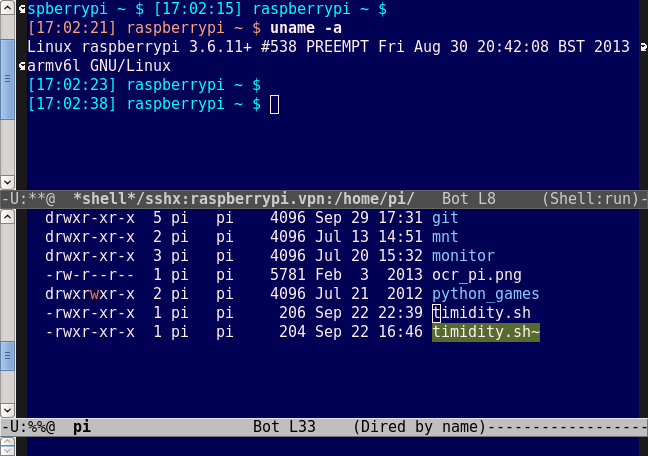
\includegraphics[width=12cm]{image201311/tramp-screenshot.png}


\subsection{$B%j%b!<%H%[%9%HB&$N@_Dj(B}
ssh $B$G@\B3$5$l$kB&$N$N@_Dj$G$9$,!"(Btramp$B$O%7%'%k$N%;%C%7%g%s$NF~=PNO$rMxMQ$7!"5!3#E*$K(B
$B%W%m%s%W%H$r8!=P$9$k$N$G!"%W%m%s%W%H!J(BPS1$B$J$I!K$r%+%9%?%^%$%:$7$F$$$k$H(B
$BF0$+$J$$>l9g$,$"$j$^$9!#(Btramp$B$N$?$a$K!!(B\texttt{.bashrc}$B$O%7%s%W%k$K$9$k$H$$$$$+$b(B
$B$7$l$^$;$s!#(B

$BNc$($P!"(Braspbian $B$N%G%U%)%k%H$O?'$,$D$-$^$/$C$F$?$j$7$F%U%!%s%7!<2a$.$F$&(B
$B$^$/F0$-$^$;$s$G$7$?!#(B

\subsection{ssh$B$N@_Dj$H%A%e!<%K%s%0(B}

$B%m!<%+%k$N(Bssh$B$N@_Dj%U%!%$%k(B \verb!~/.ssh/config! $B$K@_Dj$7$?$[$&$,$h$$$b(B
$B$N$r>R2p$7$^$9!#(B
$B%^%K%e%"%k$O(B \verb!man ssh_config!\cite{sshconfig}$B$G;2>H$G$-$^$9!#(B

\subsubsection{ControlMaster$B$G@\B3$r:FMxMQ(B}

$B<j85$G$O$3$s$J@_Dj$K$7$F$$$^$9!#(B

\begin{commandline}
 ControlMaster auto
 ControlPersist 120
 ControlPath ~/tmp/ssh-%r@%h:%p
\end{commandline}


ControlPersist $B$K;XDj$7$?IC?t4V!"(Bssh$B$G@\B3$9$k:]$K%G!<%b%s%W%m%;%9$,5/F0(B
$B$7$F!"%3%M%/%7%g%s$rD%$j$C$Q$J$7$K$7!"%3%M%/%7%g%s$r:FMxMQ$7$F$/$l$^$9!#(B

$B<j85$G$O!"(BControlPath$B$rL@<(E*$K;XDj$7$F$$$^$9!#%[!<%`%G%#%l%/%H%j0J2<$N(B
tmp $B0J2<$K$7$F$$$k$N$O%U%!%$%kL>$,M=A[2DG=$K$J$k$N$G>WFM$rKI$0$?$a$G$9!#(B

ControlMaster$B$r(BAuto$B$K$7$F$*$/$H$9$G$K%3%M%/%7%g%s$,3+$$$F$$$J$$>l9g$O%G!<(B
$B%b%s$r$?$A$"$2$F!"$b$7%3%M%/%7%g%s$,3+$$$F$$$k>l9g$K$O$=$l$rMxMQ$9$k$h$&(B
$B$K$J$j$^$9!#(B

$B%j%b!<%H$G(Btrue$B%3%^%s%I$r<B9T$9$kB.EY$r7WB,$7$F$_$?$H$3$m(B
$B?oJ,9bB.$K$J$j(B(\fgref{fig:pingwagner})$B!"(Bping time $B$NFsG\$/$i$$$K$J$C$F$/$l(B
$B$k$h$&$G$9!#(B

\begin{table}[ht]
\begin{center}
  \begin{tabular}{|c|c|}
   command & time(ms) \\
   ping& 271 \\
   ssh connection sharing on & 544 \\
   ssh connection sharing off & 4070 \\
 \end{tabular}
 \caption{ping test against wagner.debian.org}
 \label{fig:pingwagner}
\end{center}
\end{table}

\subsubsection{keep-alive}

tramp$B$O%M%C%H%o!<%/@\B3$N@ZCG$r(Bssh$B%W%m%;%9$N@8;`$G8!=P$7$^$9!#(B
ssh$B$O%M%C%H%o!<%/@\B3$,$-$l$?$j$7$F$b$9$0$K$O$=$l$r8!=P$7$J$$$N$G!"%-!<(B
$B%W%"%i%$%V$rAw?.$9$k$h$&$K$7$^$9!#(B

\begin{commandline}
 ServerAliveInterval 3
 ServerAliveCountMax 5
\end{commandline}


$BK\Ev$O%Q%=%3%s$,%5%9%Z%s%I$+$iI|3h$7$F?7$7$$%M%C%H%o!<%/@\B3$K$D$J$,$C$?(B
$B$i(Bssh$B%W%m%;%9$K:F@\B3$7$F$[$7$$$N$G$9$,!"$=$NJ}K!$r$^$@H/8+$G$-$F$$$^$;(B
$B$s!#(B

\subsubsection{$B$=$NB>$N@_Dj(B}

Mac $B$N(BRendezvous$B$H$+(BLinux$B$N(BAvahi$B$H$+@_Dj$7$F$$$k$H%[%9%HL>(B.local $B$H$$$&L>(B
$BA0$GL>A02r7h$,$G$-$k$h$&$K$J$j$^$9$,!"$=$&$9$k$H(BIP$B%"%I%l%9$O(BDHCP$B$@$H0lDj(B
$B$G$O$J$$$?$a!"(BIP$B$KBP$7$F$N80$,0c$&$HE\$i$l$^$9!#$=$N>l9g$O%[%9%H(BIP$B$r%A%'%C(B
$B%/$7$J$$$h$&$K$9$k$H$h$$$G$7$g$&!#(B

\begin{commandline}
 Host *.local
  CheckHostIP no
\end{commandline}

$B$"$H%G%U%)%k%H$G$O$$$m$$$m$J80$r;n$7$?$j$9$k@_Dj$K$J$C$F$$$^$9$,!"$D$$$G(B
$B$K80$r;XDj$7$F8x3+80G'>Z$K$7$F$*$/$H$h$$$s$8$c$J$$$G$7$g$&$+!#(B

\begin{commandline}
 Host raspberrypi.vpn
  Hostname $B$=$N%[%9%H$N(BIP$B%"%I%l%9(B
  IdentityFile ~/.ssh/ssh-keygen$B$G:n$C$?%U%!%$%k$N%Q%9(B
  IdentitiesOnly yes
\end{commandline}


\subsection{tramp$B$N(B.emacs $B$G$N@_Dj$H%A%e!<%K%s%0(B}

\texttt{.emacs} $B$K$[$H$s$I@_Dj$7$J$/$F$b%G%U%)%k%H$N@_Dj$G$=$l$J$j$K$&$4(B
$B$-$^$9!#(B
$B%^%K%e%"%k$O(B info $B7A<0$GDs6!$5$l$F$$$^$9(B\cite{trampinfomanual}$B!#(B

tramp$B$G$O(B\texttt{/sudo:root@hostname:/} $B$N$h$&$J7A<0$G%j%b!<%H%[%9%H>e$G(B
sudo$B$GJL%f!<%6$K$J$C$F$+$i%U%!%$%k$K%"%/%;%9$9$k$h$&$K;XDj$9$k$3$H$,2DG=(B
$B$G$9!#$?$@!"$=$N$?$a$K$O%j%b!<%H%[%9%H$X$NE~C#<jCJ$r;XDj$9$kI,MW$,$"$j$^(B
$B$9!#$?$H$($P!"%m!<%+%k%M%C%H%o!<%/$K$"$k%[%9%H(B \texttt{*.local} $B$G(Bsudo$B$r(B
$B%5%]!<%H$7$?$$$H$$$&MWK>$G$"$l$P!"<!$N$h$&$J@_Dj$rDI5-$7$F$*$-$^$9!#(B

\begin{commandline}
 (add-to-list 'tramp-default-proxies-alist
      '("\\.local\\'" "\\`root\\'" "/ssh:%h:"))
\end{commandline}

$B$"$H!"%G%U%)%k%H$N@_Dj$@$H%j%b!<%H%"%/%;%9$7$F$$$k$H$$$&%a%C%;!<%8$,%9%F!<(B
$B%?%9$KI=<($5$l$k$N$G$9$,!"@5D><YKb$J$N$G$=$l$r>C$9$N$b$h$$$+$H;W$$$^$9!#(B

\begin{commandline}
(custom-set-variables '(tramp-verbose 1))
\end{commandline}

\begin{thebibliography}{0}
 \bibitem{trampinfomanual} ``TRAMP User Manual'', info
	 page,
	 \url{http://www.gnu.org/software/emacs/manual/html_node/tramp/index.html#Top}
 \bibitem{sshconfig} ``ssh\_{}config(5)'' manual page,
\end{thebibliography}
%-------------------------------------------------------------------------------
\dancersection{asterisk$B@_Dj(B}{$B>e@n=c0l(B}
%-------------------------------------------------------------------------------
\index{asterisk}

% \printindex

\cleartooddpage

\vspace*{15cm}
\hrule
\vspace{2mm}

\includegraphics[width=2cm]{image200502/openlogo-nd.eps}
\noindent \Large \bf Debian $BJY6/2q;qNA(B\\
\noindent \normalfont \debmtgyear{}$BG/(B\debmtgmonth{}$B7n(B\debmtgdate{}$BF|(B \hspace{5mm}  $B=iHGBh(B1$B:~H/9T(B\\
\noindent \normalfont $BEl5~%(%j%"(B Debian $BJY6/2q(B $B!JJT=8!&0u:~!&H/9T!K(B\\
\hrule

\end{document}
